\documentclass[12pt, a4paper]{article} %Definerer skriftstørrelse, arktrype( eks a0paper, ..., a6paper, letterpaper....), dokumenttype(article, report, book, letter, beamer(presentasjon).   
\usepackage[font=small, labelfont=bf]{caption}
\usepackage{graphicx}
\usepackage{amsmath, amssymb} %  matematiske funskjoner og symboler. 
\usepackage{listings}
\usepackage{url} % urls in the bibliograpy
\usepackage[utf8]{inputenc} % 
\usepackage{float}  %
\usepackage{subcaption} % NOT compatible with the subfig package
\usepackage{authblk}
\usepackage{siunitx}
\usepackage[]{algorithm2e}



\usepackage[ 
%total={250mm,297mm},  
left=25mm,
 right=25mm,
 top=30mm,
 bottom=20mm]{geometry} % kan endre på marger 
%%%%%%%%%%%%%%%%%%%%%%%%%%%%%%%%%%%%%%%%%%%%%%%%%%%%%%%%%%%%%%%%
% Gode infosider:
% https://no.sharelatex.com/learn/Creating_a_document_in_LaTeX 
% https://no.sharelatex.com/learn/Page_size_and_margins
 
%%%%%%%%%%%%%%%%%%%%%%%%%%%%%%%%%%%%%%%%%%%%%%%%%%%%%%%%%%%%%%%%
% Det som inkluderes i \maketitle
\title{Solving the poisson problem on supercomputer \\
TMA4280: Introduction to Supercomputing}
\author[]{Jon Christian Halvorsen, Monica Kappelslåen Plassen \\and Anette Fossum Morken}
\date{}
%%%%%%%%%%%%%%%%%%%%%%%%%%%%%%%%%%%%%%%%%%%%%%%%%%%%%%%%%%%%%%%
\begin{document}
\maketitle
\RestyleAlgo{boxruled}
%\begin{abstract}

%\end{abstract}
\section*{Introduction}
In this project, we have been studying the two-dimensional Poisson problem, and a discrete solver based on diagonalization and the Discrete Sine Transform. A serial code was parallelized using MPI and OpenMP, the correctness of the solution was verified and the program tested on the cluster Kongull. 

\section*{Theory}
In this project we are studying the two-dimensional Poisson problem
\begin{align}\\
\label{Poisson}
-\nabla^2u&=f \quad\quad\text{ in } \Omega=(0,1)\times(0,1)\\
u&=0 \quad\quad\text{ on } \partial \Omega, \nonumber
\end{align}
where $f$ is given load function and $u$ is the solution. We have been using two different load functions
\begin{align*}
f(x,y)&=1
\end{align*}
and
\begin{align}
\label{loadfunc2}
f(x,y)&=5\pi^2\sin(2\pi x)\sin(\pi y) \quad\text{with exact solution} \\
u(x,y)&=\sin(2\pi x)\sin(\pi y).\nonumber
\end{align}
We discretize the Laplace operator with the five-point stencil and use regular finite difference grid with $(n+1)$ points, and therefore $h = \frac{1}{n}$ spacing, in each direction and, at first, a global numbering scheme. This results in a SPD algebraic system
\begin{equation}
	\mathbf{Au} = \mathbf{b}
	\label{system1}
\end{equation}
where $\mathbf{b}$ is found from the loading function times the term $h^2$. $\mathbf{A}$ is a tensor product operator $\mathbf{A} = \mathbf{I}\bigotimes\mathbf{T} + \mathbf{T}\bigotimes\mathbf{I}$ where $\mathbf{T}$ is the matrix from the one dimensional Poisson problem. Thus, using a local numbering scheme, \eqref{system1} can be stated as 
\begin{equation}
	\mathbf{TU} + \mathbf{UT} = \mathbf{B}
\end{equation}
We know that $\mathbf{T}$ is SPD, thus we can perform an eigendecomposition $\mathbf{T} = \mathbf{Q\Lambda Q^T}$. Now, letting $\mathbf{\widetilde{B}} = \mathbf{Q^TBQ}$ and $\mathbf{\widetilde{U}} = \mathbf{Q^TUQ}$, we finally arrive at the system 
\begin{equation}
	\mathbf{\Lambda\widetilde{U}} + \mathbf{\widetilde{U}\Lambda} = \mathbf{\widetilde{B}}.
	\label{system2}
\end{equation}
Finding $\mathbf{\widetilde{U}}$ from \eqref{system2} is a simple calculation when we know the eigenvalues of $\mathbf{T}$, and we can from this get the final answer $\mathbf{U}$. Now we utilize what we know about the Poisson problem to avoid the two matrix-matrix products needed to compute both $\mathbf{\widetilde{B}}$ and $\mathbf{\widetilde{U}}$, which requires $\mathcal{O}(N^3)$ time. \\
\\
We utilize the fact that we know the eigenvalues $\lambda$ and eigenvectors $\mathbf{q}$ of $\mathbf{T}$, in particular the eigenvectors and the eigenvalues are
\begin{align*}
	(q_j)_i &= \sqrt{\dfrac{2}{N}}\sin \Big( \dfrac{ij\pi}{N}\Big) \\
	\lambda_i &= 2\left(1-\cos\left(\frac{i \pi}{N}\right) \right),
\end{align*}
which lead to the following solution to system (\ref{system2}):
\begin{align*}
\tilde{u}^T_{i,j} &= \frac{\tilde{b}^T_{i,j}}{\lambda_i + \lambda_j}, 1 \leq i, j \leq N
\end{align*}
\\ \\
Notice that these eigenvectors (if normalized) are the same as the basis for the discrete sine transform, given in the lecture slides. \cite{forelesning} Thus, we can use the DST to find $\mathbf{\widetilde{B}}$ and $\mathbf{U}$. Let $\mathbf{S}$ denote the discrete sine transform, and $\mathbf{S}^{-1}$ be the inverse transform. We can now express $\mathbf{Q} = \sqrt{\frac{N}{2}\mathbf{S}}$ and $\mathbf{Q}^T = \sqrt{\frac{2}{N}}\mathbf{S}^{-1}$, and therefore $\mathbf{\widetilde{B}}^T = \mathbf{S}^{-1}((\mathbf{SB})^T)$ and $\mathbf{U} = \mathbf{S}^{-1}(\mathbf{S}(\mathbf{\widetilde{U}}^T))^T$. Both of these operations can be done in $\mathcal{O}(N^2\log{N})$ time. 
This leads us to the following serial code:\\

\begin{algorithm}[H]
 \KwData{$\mathbf{B}$, load matrix.}
 \KwData{$\mathbf{S}$ the discrete fourier transform operator.}
 \KwResult{$\mathbf{U}$, solution matrix. }
 Calculate $\mathbf{\widetilde{B}}^T = \mathbf{S}^{-1}((\mathbf{SB})^T)$  \;
 Solve system (\ref{system2}): $\tilde{u}^T_{i,j} = \frac{\tilde{b}^T_{i,j}}{\lambda_i + \lambda_j}, 1 \leq i, j \leq N$\;
 Calculate $\mathbf{U} = \mathbf{S}^{-1}((\mathbf{S}\mathbf{\tilde{U}}^T)^T)$ \;
 \caption{Pseudocode for serial poisson solver using discrete sine transform.}
 \label{code:serial}
\end{algorithm}

\section*{Parallelization}
Converting the serial code in algorithm \ref{code:serial} to parallel is split in two parts, one part for using MPI and one part for using openMP. Since the MPI code needs most drastic change we start with that.

\subsection*{MPI parallelization}
Inspection of the code in algorithm \ref{code:serial} reveals the following tricks that enable us to write parallel code from the start to the end: (in the following a node is referred to as one MPI processor)
\begin{itemize}
\item Each node can compute the needed part from $\textbf{B}$.
\item The whole $\lambda$ vector is needed in each node given that we split $\textbf{B}$ column or row wise.
\item Given the above two points, the only time we need to exchange data from node to node is in the transpose function (and when we gather the results).
\end{itemize}

The new pseudocode for our parallel code then becomes:

\begin{algorithm}[H]
 \KwData{$b(x,y)$ The load function.}
 \KwData{$\mathbf{\widetilde{X}}$, buffer to store intermediate results.}
 \KwData{$\mathbf{S}$ the discrete fourier transform operator.}
 \KwResult{$\mathbf{U}$, solution matrix. }
 Generate submatrix of $\textbf{B}$ for this node using the function $b(x,y)$\;
 Generate the whole vector $\lambda$ \;
 Let $\mathbf{\widetilde{X}} = \mathbf{SB}$  \;
 Let $\mathbf{\widetilde{X}}^T = $parallel\_transpose($\mathbf{\widetilde{X}}$)   \;
 Let $\mathbf{\widetilde{B}}^T = \mathbf{S}^{-1}(\mathbf{\widetilde{X}}^T)$ \;
 Solve system (\ref{system2}): $\tilde{u}^T_{i,j} = \frac{\tilde{b}^T_{i,j}}{\lambda_i + \lambda_j} 1 \leq i, j \leq N$\;
 Let $\mathbf{\widetilde{X}}^T = \mathbf{S}\mathbf{\tilde{U}}^T$  \;
 Let $\mathbf{\widetilde{X}} = $parallel\_transpose($\mathbf{\widetilde{X}}^T$)   \;
 Let $\mathbf{U} = \mathbf{S}^{-1}(\mathbf{\widetilde{X}}) $ \;
 Gather the results from all nodes into the big $\mathbf{U}$.
 \caption{Pseudocode for serial poisson solver using discrete sine transform.}
 \label{code:parallel}
\end{algorithm}

with the parallel\_transpose function as follows.

\begin{algorithm}[H]
 \caption{Parallel\_transpose function. Notice that it returns a matrix of the same dimension as its input.}
 \KwData{Matrix $\mathbf{X}$ with $n$ rows and $m \leq n$ columns.}
 \KwResult{Matrix $\mathbf{Z}$ with $n$ rows and $m \leq n$ columns.}
 Determine which elements in $\mathbf{X}$ should go which nodes and order linearly in memory \;
 Spread out all elements to the correct nodes \;
 Get new elements from other nodes \;
 Order the elements correctly in memory according to a transpose operation and return as $\mathbf{Z}$.
 \label{code:transpose}
\end{algorithm}
We split the load matrix column wise and notices that the parallel\_transpose function preserves the nice data structure on each node. We chose to implement the sending and receiving of data in the transpose function as an MPI\_Alltoallv call after laying out the elements in a correct linear layout first. Unpacking the data after the MPI call is just using the same structure to get it back, only remembering that we need to transpose the data.

Furthermore, the gathering of data into one big $\mathbf{U}$ is not really necessary. We could either use MPI\_IO to write to disk or we're not interested in the matrix at all (say you're interested in the error or the computation time) we can just return that instead. All in all, this should be a really effective parallelization of the serial code since we severely limit the amount of network operations we have to do (only two MPI\_Alltoallv and one MPI\_Gather if we need result).

\subsection*{OpenMP parallelization}
 
\section*{Hardware}
Our code is run on the Kongull which is a linux cluster using CentOS 5.3 and running Rocks. The cluster has 1 login node, 4 I/O nodes and 108 compute nodes. 96 of the compute nodes have two 6-core AMD Istanbul processors while the 12 last nodes have 2 8-core Intel Sandy Bridge processors. For more information about the cluster we refer to the clusters webpage \cite{kongull}. 
 
\section*{Convergence analysis and testing}
To check convergence we run the poisson solver with the load function and exact solution given in equation (\ref{loadfunc2}). We run the \textit{wrapper\_n.sh} script on kongull to run the exact same configuration 11 times with only $n$ changing each iteration. We let $n$ vary from $2^4$ to $2^{14}$. We run the job with 3 openMP threads and 12 MPI processors. The program returns the maximum error over the whole domain. This is then imported to matlab and plotted on the logarithm scale in figure \ref{fig:checkConv}. For the given test data we have quadratic convergence as expected.


\begin{figure}[h]
\centering
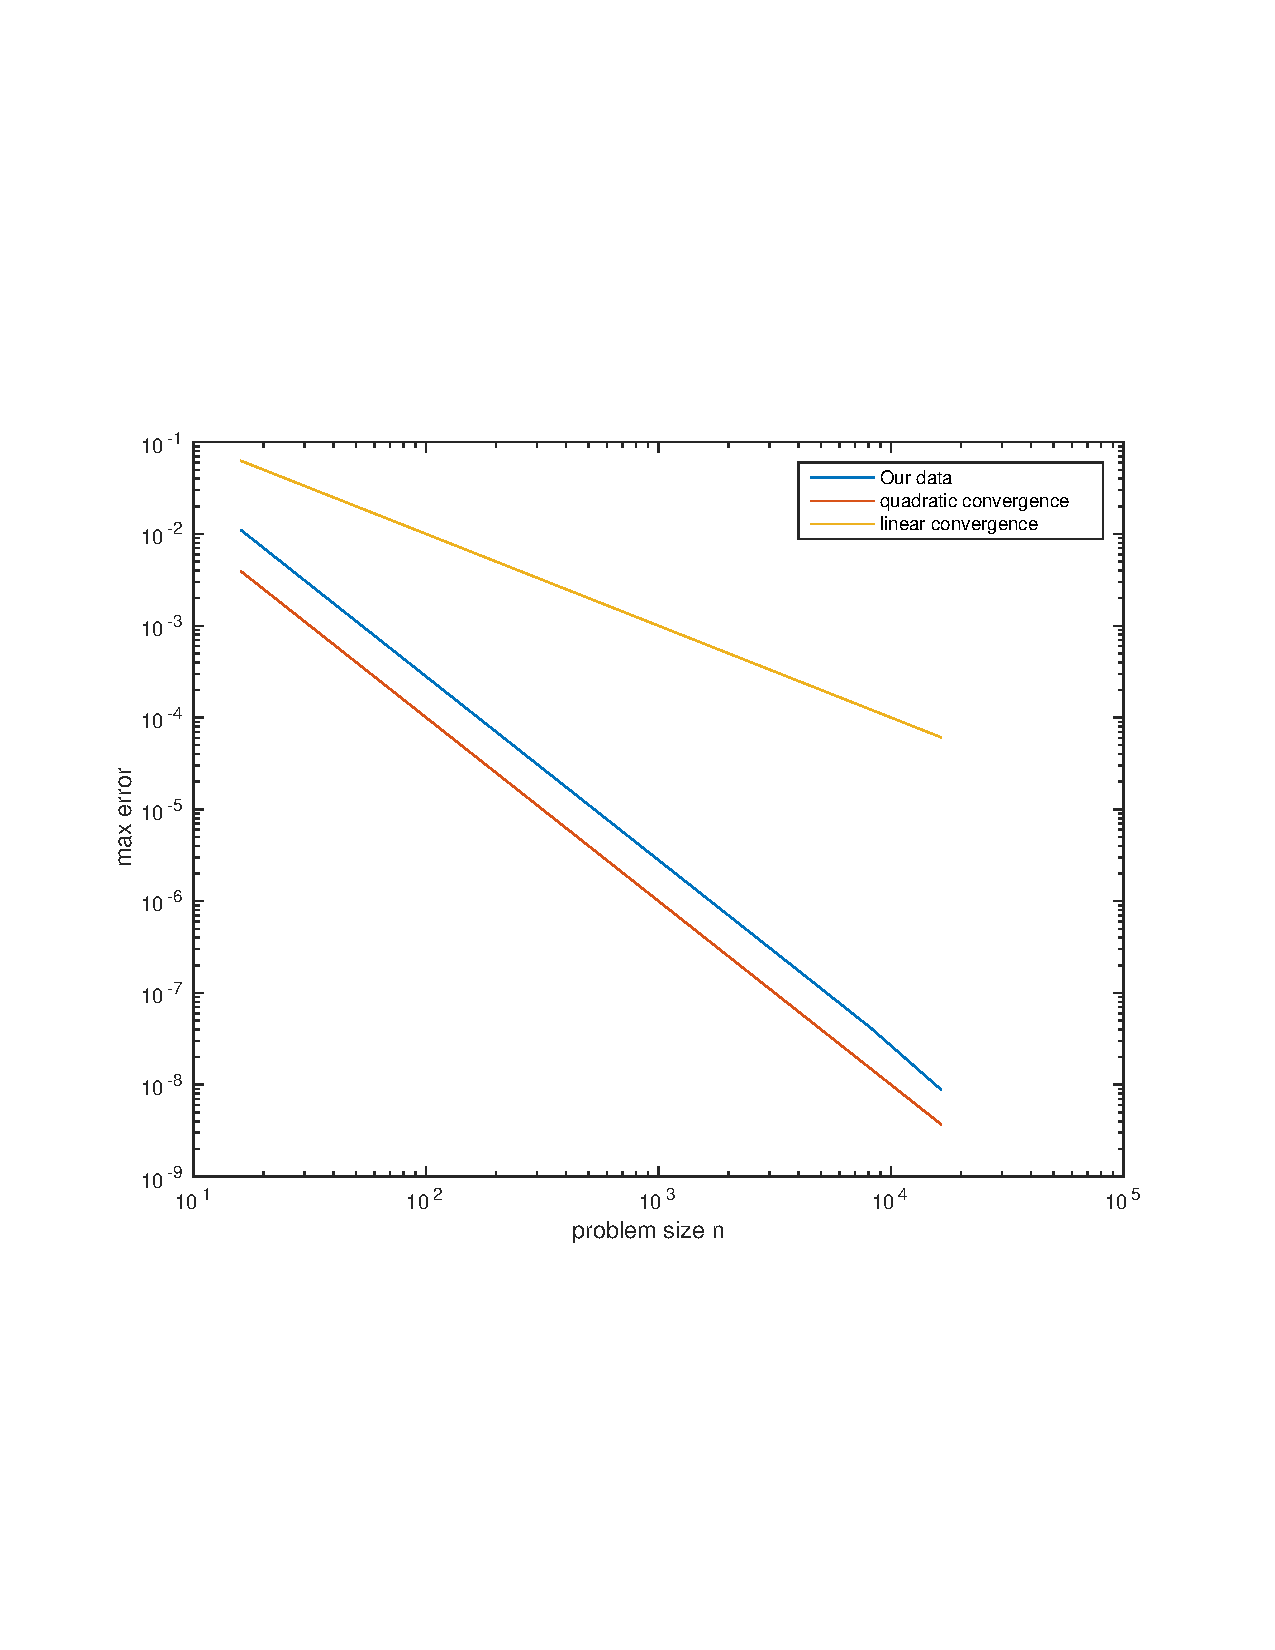
\includegraphics[width=0.6\linewidth]{./figures/checkConv}
\caption{Shows that the result from the convergence test compared with curves with slope $h$ and $h^2$}
\label{fig:checkConv}
\end{figure}

\section*{Results}
\subsection*{Running only MPI or openMP}
\begin{figure}[h!]
			\centering
			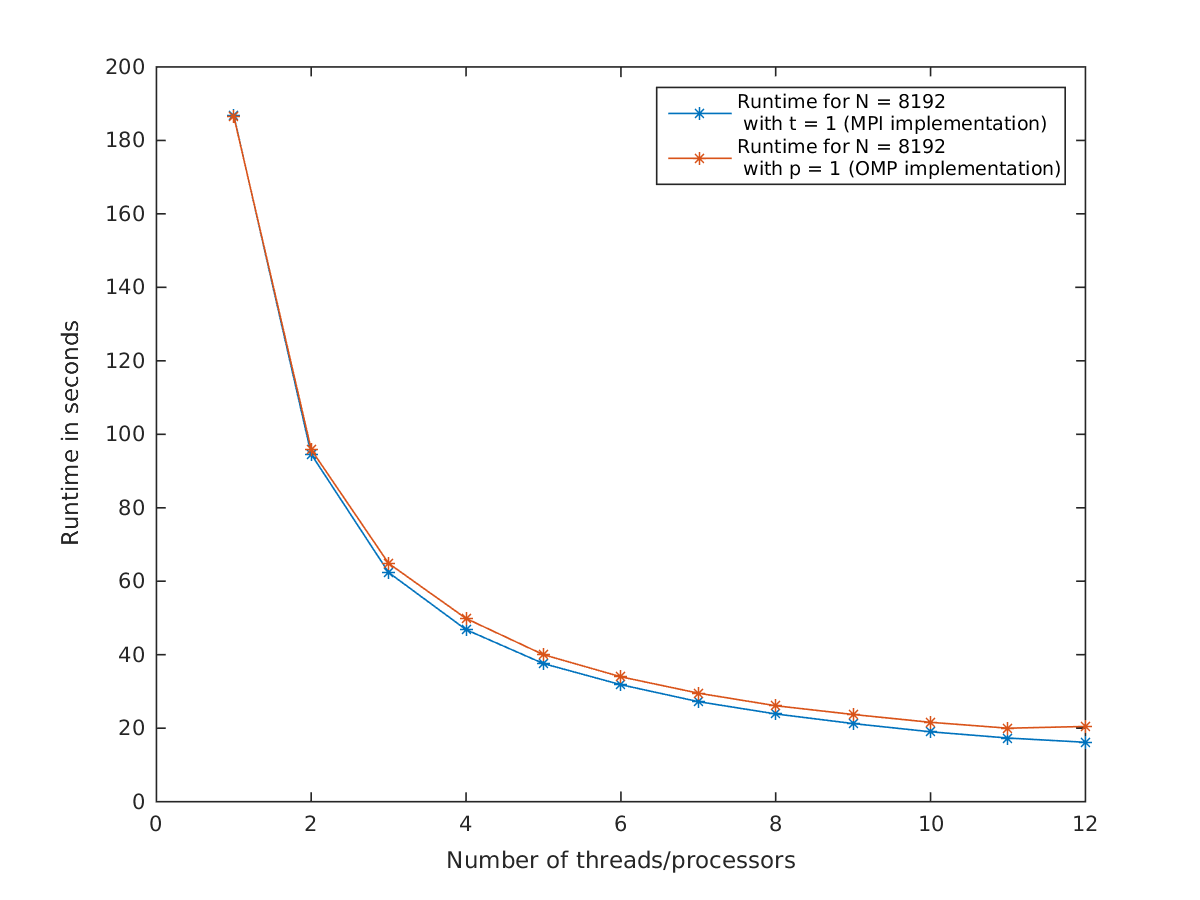
\includegraphics[width=0.7\textwidth]{./figures/runtime_either_MPI_OMP}
			\caption{Runtime for MPI and OMP program.}
			\label{fig:MPIvsOMP}
\end{figure}
We first run our code both as a pure MPI and as a pure OpenMP program on one node to look at runtime. From figure \ref{fig:MPIvsOMP} we see that the runtime is equal for $t = p = 1$, as it obviously should be since this is the serial implementation. Then, the runtime decreases as $p$ and $t$ increases, as it should. In other words, we get a good speedup for both parallelization methods given that we are one one node. 


\subsection*{Optimal number of nodes with MPI}

The next question then becomes: given a number of processors, which number of nodes will work best? The results are presented in figure \ref{fig:bestnodes}.
\begin{figure}[h]
\centering
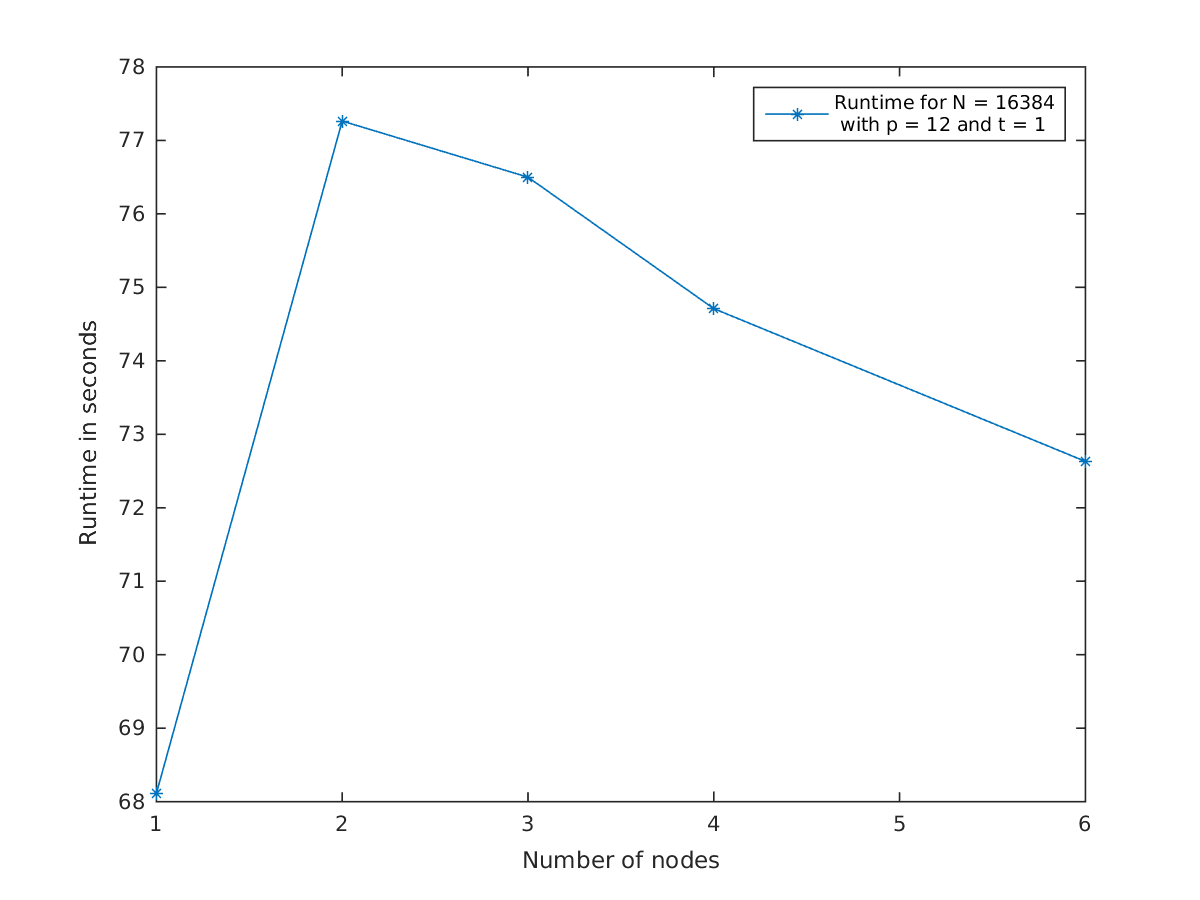
\includegraphics[width=0.7\textwidth]{./figures/bestnodes}
\caption{Running the problem on a different amount of nodes with the combined number of processors to be 12.}
\label{fig:bestnodes}
\end{figure}
The clearly best result is if we keep all the processing on a single node, but the moment we spread out to two or more nodes we get a speedup for every new node we add (at least till six nodes). We attribute this be the limiting factor of bandwidth between the nodes. We will get much more efficient use of the bandwidth if we spread our data across multiple nodes. The implementation only transfers data in the transpose function, but then again it transfers a lot of data at the same time and it is natural that we reach the bandwidth cap.


\subsection*{Hybrid vs pure distributed memory model}
To test the hybrid and the pure distributed memory model we do a few runs on Kongull with the following settings such that $n = 16384$,  $t\cdot p = 36$ and $p = \{1, 2, 3, 4, 6, 9, 12, 18, 36\}$.
\begin{figure}
\centering
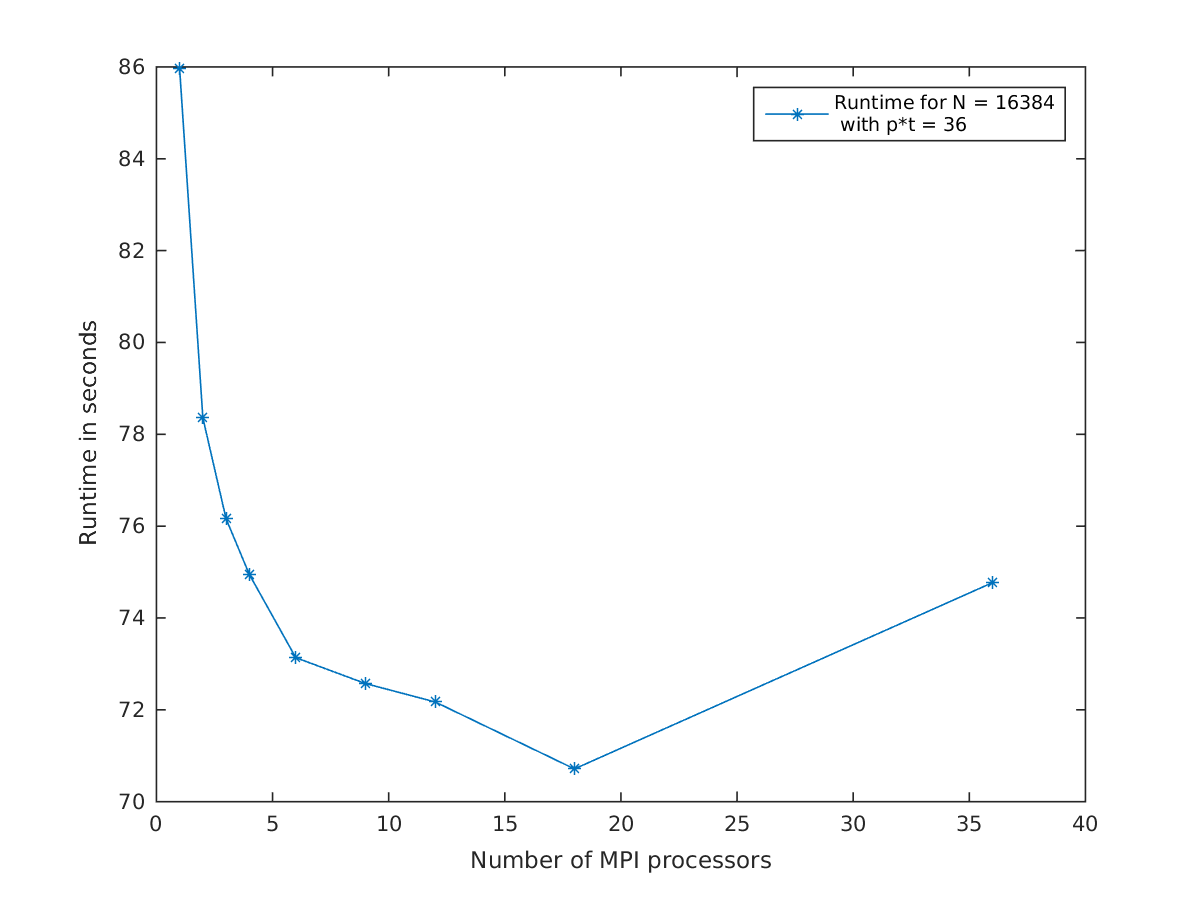
\includegraphics[width=0.7\textwidth]{./figures/pt36}
\caption{Runtime with different numbers for MPI processors and openMP threads with $p\cdot t = 36$.}
\label{fig:runtime}
\end{figure}
As seen in figure \ref{fig:runtime} the pure distributed model outclasses the hybrid model. This may be the case since the problem is pretty local in the sense that we don't need many MPI calls. We need, however, quite a few openMP calls. It seems reasonable that for this problem the pure distributed memory model works best since we only need to send data between nodes twice, and it may be most efficient to just spread the data all the way from the beginning. More testing shows that even when just using one node (and twelve cores) the pure distributed model performs marginally better than the hybrid model.


\subsection*{Speedup and parallel efficiency}
The speedup, $S_P$ is is defined as the ratio between the solution time on one single processor divided by the solution time on $P$ processors, $S_p=\frac{T_1}{T_P}$. Ideally $S_P$ should be $S_P=T_1P$. When we study figure \ref{fig:speedup}, that is the plot of the speedup of our code, we see that in the beginning this happens, but with more that with more processors the speedup still increases, but not as much.
\\ \\
The speedup increases because the all computational tasks are spread to all the processors so the computing task for each processor is reduced. When the problem increases and the number of processors increases the communication between the processors increases. At one point the time used to communicate increases so much that it reduces the run time the speedup. We have not yet encountered this, but we assume it'll come soon if we continue to increase the problem size.

\begin{figure}
        \centering
        \begin{subfigure}[b]{0.45\textwidth}
			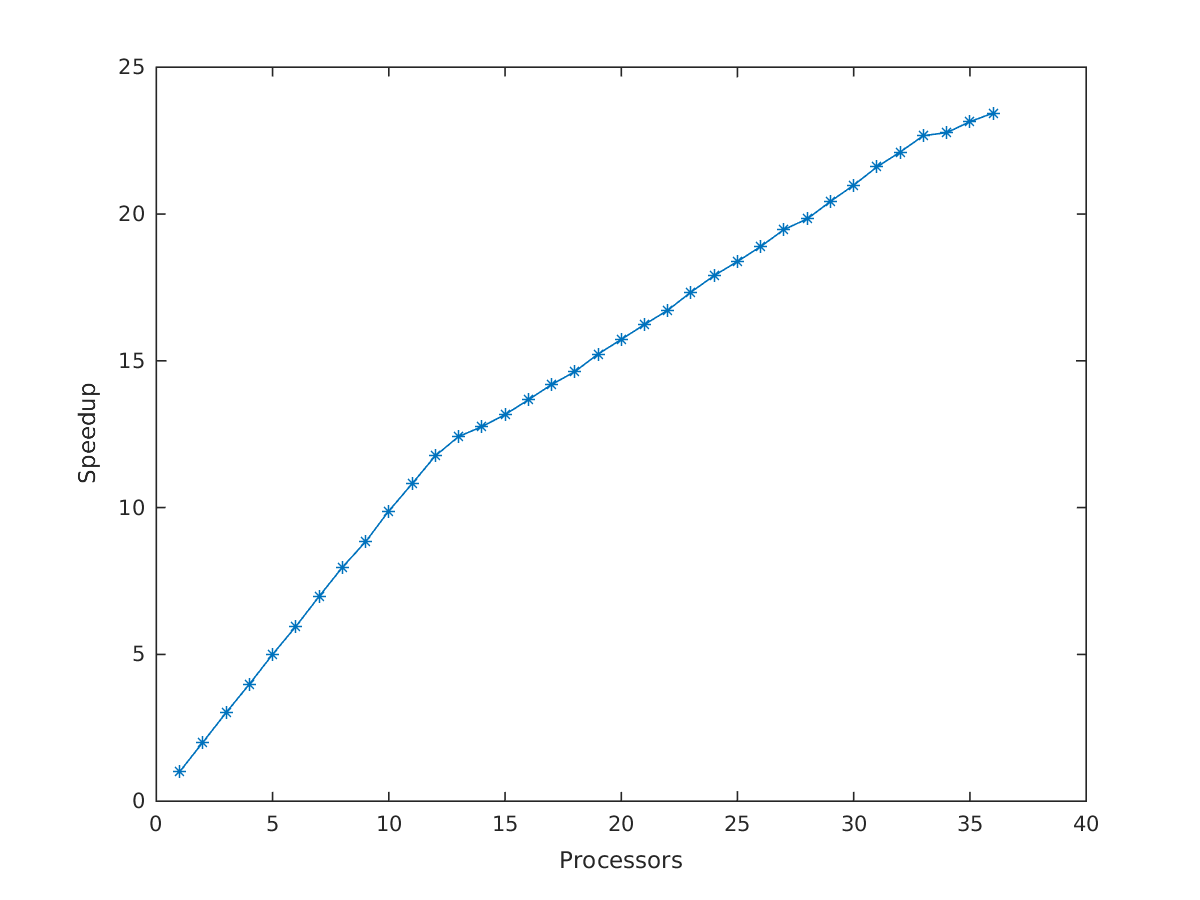
\includegraphics[width=\textwidth]{./figures/speedup}
			\caption{Parallel speedup.}
			\label{fig:speedup}
        \end{subfigure}
        ~ %add desired spacing between images, e. g. ~, \quad, \qquad, \hfill etc.
          %(or a blank line to force the subfigure onto a new line)
        \begin{subfigure}[b]{0.45\textwidth}
			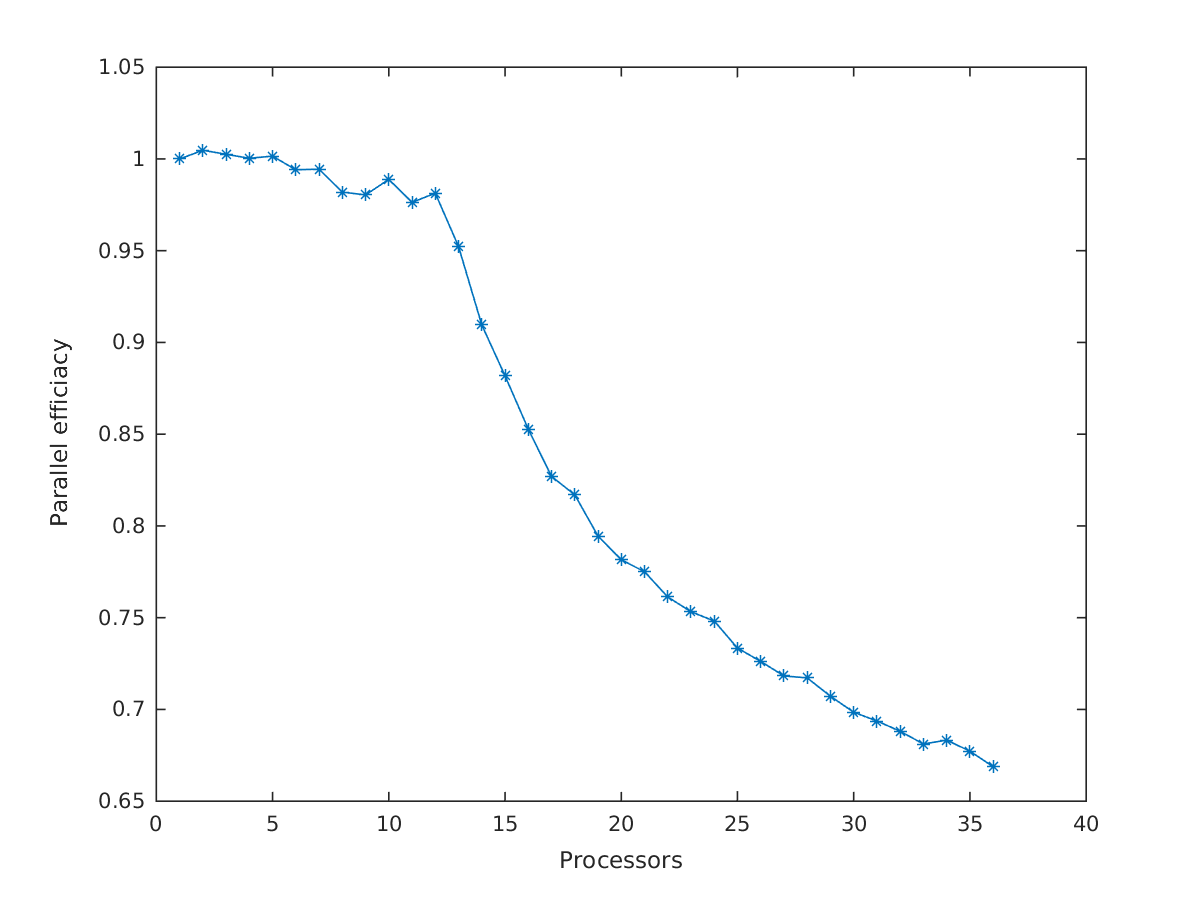
\includegraphics[width=\textwidth]{./figures/efficiacy}
			\caption{Parallel efficiency.}
			\label{fig:efficiacy}
        \end{subfigure}%
        \caption{Parallel speedup and efficiency for the pure distributed memory model}
        \label{fig:analysis}
\end{figure}

As can be seen in figure \ref{fig:efficiacy} the parallel efficiency, defined as $\eta_P=\frac{S_P}{p}$, is almost ideal as long we only use a single node with 12 processors. With more than 12 processors the efficiency drops, but the speedup still makes it worth it. We assume this happens because the network overhead of using more than one node inhibits the efficiency more than the overhead of transporting things inside the node itself. According to the model linear model of data transfer latency we would say that the latency (the constant) is larger when communicating between nodes than when we communicate in-node.


\subsection*{How does runtime scale with N}
\begin{figure}[h!]
			\centering
			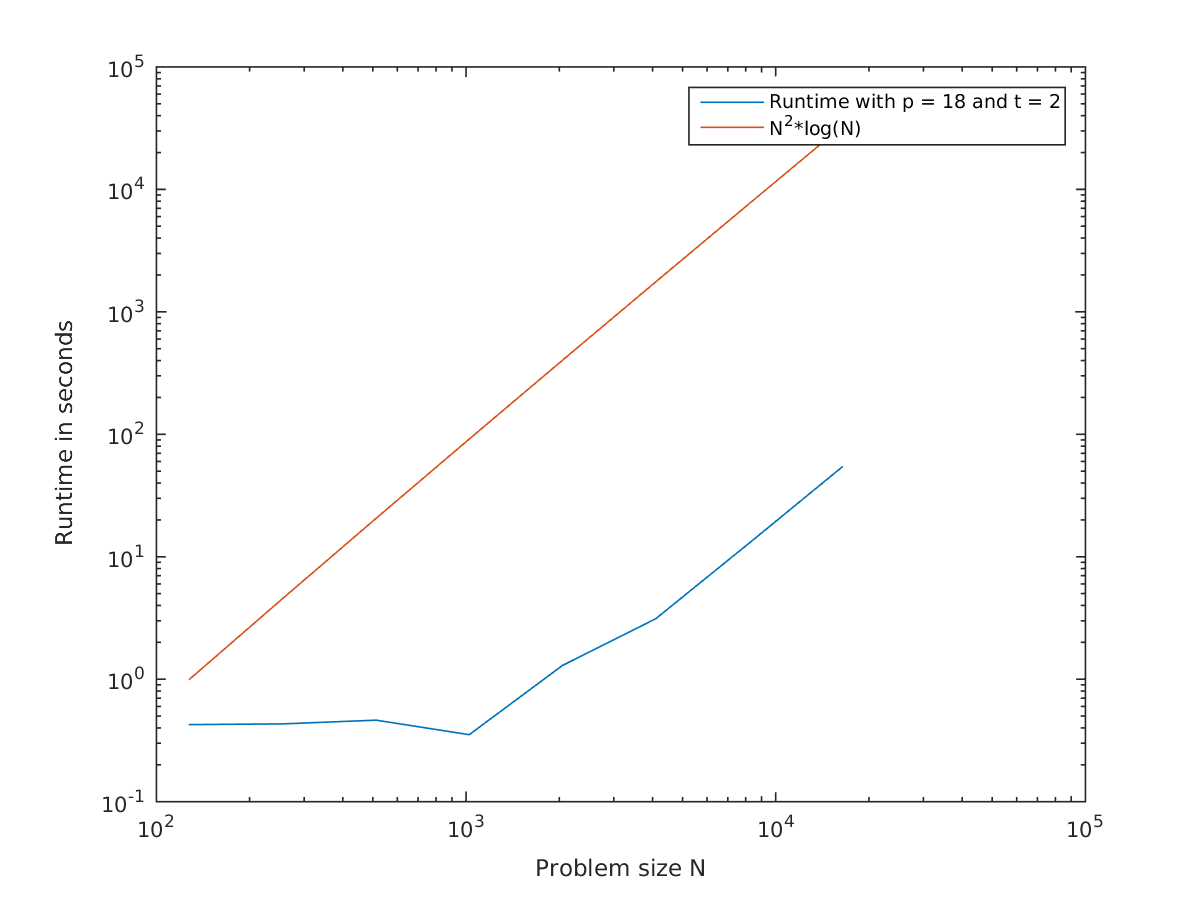
\includegraphics[width=0.7\textwidth]{./figures/runtimeN}
			\caption{Runtime with increasing problem size.}
			\label{fig:runtimeN}
\end{figure}
Next, we study how the runtime of our program scales with the problem size $N$. From the theory, we know that the runtime should be of order $\mathcal{O}(N^2\log(N))$. We observe from figure \ref{fig:runtimeN} the runtime appear to go towards the expected order as $N$ increases. 


\section*{Discussion}
\subsection*{Choosing a different loading function}
When going from the simple case of the loading function being identically $1$, to it being a different function we need to evaluate the function in the point corresponding to the element we are in. For the whole matrix, the assignment is done by
\begin{align*}
	(B)_{i,j} = h^2\cdot f\Big(\frac{i}{N},\frac{j}{N}\Big) \quad \text{for } i,j = 1,...,N-1.
\end{align*}
In the parallel code, it is important to make sure that each node is able to map its elements to the correct corresponding points on the grid when evaluation the function $f$. This is done by using what we know about which, and how many, columns each node has.

\subsection*{Different boundary conditions}

So far, we have only considered homogenous Dirichlet boundary conditions. In the case of non-homogenous Dirichlet boundary conditions, the load matrix $\mathbf{B}$ would be different. Most of $\mathbf{B}$ would be as before, but the first and last rows and columns should contain the boundary point information from the discretization. \\
\\
We could have implemented the boundary condition in this way: each node gets the boundary value information, and apply the boundary conditions of the rows. Since it is known how many nodes the program uses, we can tell the first and the last node separately to apply the boundary conditions for the columns(for the first node it applies the boundary condition in the first column and the last node applies the boundary conditions in the last column).

\subsection*{Choosing a more complex domain}

We have also assumed that the domain is the unit square. If this was not the case, but we instead had had a rectangle with sides $L_x$ and $L_y$, i.e. $ \Omega = (0,L_x)\times (0,L_y)$, but still a regular finite grid with $(N+1)$ points in each spatial direction, we would have to use different values for the spacing, 
\begin{align*}
	h_x = \frac{L_x}{N} \quad \text{and} \quad h_y = \frac{L_y}{N}.
\end{align*}
In terms of the implementation, a few changes would have to be made. Because we still use a regular finite grid, $\mathbf{T}$ and $\mathbf{B}$ would still be $(N-1)\times (N-1)$ matrices, but now we cannot multiply the loading function with $h^2$ when creating the load matrix $\mathbf{B}$. The system \eqref{system2} would change to 
\begin{align*}
	\frac{1}{h_x^2}\mathbf{\Lambda\widetilde{U}} + \frac{1}{h_y^2}\mathbf{\widetilde{U}\Lambda} = \mathbf{\widetilde{B}}.
\end{align*}
Here, $\mathbf{\Lambda}$ and $\mathbf{\widetilde{U}}$ are the same as before, but $\mathbf{\widetilde{B}}$ is scaled with $\dfrac{1}{h^2}$. The calculation of $\mathbf{\widetilde{U}}^T$ would have to be done by
\begin{align*}
	\tilde{u}^T_{i,j} &= \frac{\tilde{b}^T_{i,j}}{\dfrac{\lambda_i}{h_x^2} + \dfrac{\lambda_j}{h_y^2}}, 1 \leq i, j \leq N-1.
\end{align*}
In total, the only things that would have to change in the implementation of the method, is the calculation of the load matrix $\mathbf{B}$ and the matrix $\mathbf{\widetilde{U}}^T$.

\subsection*{Possible bottlenecks}
Since we decide to split the matrix column wise and we have $2^k-1$ columns we'll (almost( never get a load balanced program. This way some processors must process $2k^-1$ more numbers than the others. It could be possible to split this in another way such that the processors share the load better. The computational difficulty of achieving this is however pretty big, but it probably could be done.

An obvious bottleneck is the bandwidth between the nodes in the system (as evidenced in figure \ref{fig:bestnodes}). Here we could have done some more testing. No matter the results of this, we think ordinary decency says that you should use all the computing power in the node you get access to and not to use any excess nodes because of a small performance boost.

If the resulting matrix should be stored, MPI-I/O could be used to store the matrix, but in our case we were only interested in whether or not it converged, so no need to store the data.


\section*{Conclusion}
We have been able to implement a parallel poisson solver using both OpenMP, MPI and a hybrid model, and verified its correctness. Using the cluster Kongull, runtime, speedup and efficiency tests were performed. The results of these tests show that the parallel code is faster than the serial implementation. Also, for our implementation, the pure distributed model outclasses the hybrid model when we limit the use of nodes. We suspect this is because alot of OpenMP calls has to be made compared to the two times data has to be sent using MPI calls. When we are liberal in the use of nodes the hybrid model seems to holding it's own ground. The best timing result we got was just above 25 seconds for the problem with $N=16384$ nodes in each spatial direction spread across 18 nodes, with $p=1$ and $t=2$ on each node for a total of 36 processors/threads. We could not get access to 36 nodes to test with $p=1$ and $t=1$. 

%%%%%%%%%%%%%%%%%%%%%%%%%%%%%%%%%%%%%%%%%%%%%%%%%%%%%%%%%
% REFERANSER
\begin{thebibliography}{10}
\bibitem{forelesning} Kvarving, Arne Morten \emph{Solving the linear system resulting from the Poisson problem.}
\bibitem{kongull} Hardware information about the Kongull cluster, gathered 26. mars 2015 from \\ \url{https://www.hpc.ntnu.no/display/hpc/Kongull+Hardware}
\end{thebibliography}
\end{document}
